\chapter{技术可行性分析}

\section{系统架构设计}

\subsection{逻辑架构与技术栈}
本系统基于微服务思想设计，整体架构分为表现层、业务逻辑层、数据持久层和基础设施层。
\begin{itemize}
    \item \textbf{表现层 (Presentation Layer)}: 采用 \textbf{Flutter} 框架构建跨平台移动应用，利用其声明式 UI 和 Skia 渲染引擎保证流畅的用户体验。
    \item \textbf{业务逻辑层 (Business Logic Layer)}:
          \begin{itemize}
              \item \textbf{API Gateway}: 通过 Nginx 反向代理进行负载均衡。
              \item \textbf{Core Service}: 基于 \textbf{Python Flask}，处理用户鉴权、设备管理。
              \item \textbf{Optimization Engine}: 集成 \textbf{Gurobi} 求解器，提供核心调度算法。
              \item \textbf{ML Service}: 基于 \textbf{Scikit-learn/LightGBM}，提供负荷预测服务。
          \end{itemize}
    \item \textbf{数据持久层 (Data Layer)}:
          \begin{itemize}
              \item \textbf{Google Firestore}: NoSQL 文档数据库，存储实时设备状态及日志。
              \item \textbf{Google Cloud Storage}: 对象存储，归档历史 CSV 数据及训练模型。
          \end{itemize}
\end{itemize}

\subsection{网络与部署拓扑}
系统的云端部署拓扑如图~\ref{fig:network_topo} 所示。

\begin{figure}[H]
    \centering
    \resizebox{0.75\textwidth}{!}{
        \begin{tikzpicture}[
                node distance=1.5cm,
                server/.style={rectangle, draw, fill=blue!10, rounded corners, minimum height=1cm, align=center},
                db/.style={cylinder, draw, fill=yellow!10, shape border rotate=90, aspect=0.25, minimum height=1cm, align=center},
                cloudNode/.style={cloud, draw, fill=gray!10, aspect=2, minimum width=3cm},
                arrow/.style={-latex, thick}
            ]

            % Nodes
            \node[cloudNode] (internet) {Internet};
            \node[server, below=of internet] (lb) {Load Balancer\\(Cloud Run)};
            \node[server, below left=of lb, xshift=-1cm] (flask1) {Flask Instance 1\\(Core Logic)};
            \node[server, below right=of lb, xshift=1cm] (flask2) {Flask Instance 2\\(ML/Opt)};
            \node[db, below=of flask1] (firestore) {Firestore\\(NoSQL)};
            \node[db, below=of flask2] (gcs) {Cloud Storage\\(Files)};

            % Edges
            \draw[arrow] (internet) -- (lb);
            \draw[arrow] (lb) -- (flask1);
            \draw[arrow] (lb) -- (flask2);
            \draw[arrow] (flask1) -- (firestore);
            \draw[arrow] (flask2) -- (firestore);
            \draw[arrow] (flask2) -- (gcs);

            % Box
            % Adjusted to be wider and have more margin to avoid touching Cloud Storage content
            \draw[dashed, red, thick] ($(flask1.north west)+(-0.6,0.6)$) rectangle ($(gcs.south east)+(1.0,-0.8)$);
            \node[red] at ($(flask1.north west)+(-0.6,1.0)$) {VPC Internal Network};

        \end{tikzpicture}
    }
    \caption{云端网络部署拓扑图}
    \label{fig:network_topo}
\end{figure}

\section{核心业务流程}
\subsection{智能调度交互时序}
为了明确各模块间的协作机制，图~\ref{fig:sequence} 展示了用户发起“立即优化”请求后的系统内部时序交互。

\begin{figure}[H]
    \centering
    \resizebox{0.9\textwidth}{!}{
        \begin{tikzpicture}[scale=0.8]
            \tikzstyle{block}=[rectangle, draw, fill=white, minimum width=2.5cm, minimum height=1cm]
            \tikzstyle{line}=[->, >=stealth, thick]

            % Lifelines
            \node[block, fill=blue!10] (User) {用户 (User)};
            \node[block, fill=orange!10, right=2cm of User] (App) {移动端 (App)};
            \node[block, fill=green!10, right=2cm of App] (Cloud) {云端 (API/Opt)};
            \node[block, fill=gray!10, right=2cm of Cloud] (Device) {终端 (BMS)};

            \draw[thick] (User) -- ++(0,-7);
            \draw[thick] (App) -- ++(0,-7);
            \draw[thick] (Cloud) -- ++(0,-7);
            \draw[thick] (Device) -- ++(0,-7);

            % Messages
            \draw[line] ($(User)+(0,-1)$) -- node[above, font=\scriptsize] {1. 点击优化按钮} ($(App)+(0,-1)$);
            \draw[line] ($(App)+(0,-2)$) -- node[above, font=\scriptsize] {2. POST /optimize} ($(Cloud)+(0,-2)$);

            \node[draw, dashed, inner sep=2mm, fit={($(Cloud)+(0,-2.2)$) ($(Cloud)+(0,-3.5)$)}] {};
            \node[right, font=\scriptsize, align=left] at ($(Cloud)+(0.1,-2.8)$) {3. Gurobi 求解\\(MIP Model)};

            \draw[line] ($(Cloud)+(0,-4)$) -- node[above, font=\scriptsize] {4. 下发控制策略} ($(Device)+(0,-4)$);
            \draw[line] ($(Device)+(0,-5)$) -- node[above, font=\scriptsize] {5. 执行充放电} ($(Device)+(0,-5.5)$);
            \draw[line, dashed] ($(Device)+(0,-6)$) -- node[above, font=\scriptsize] {6. 状态上报 (MQTT)} ($(Cloud)+(0,-6)$);
            \draw[line, dashed] ($(Cloud)+(0,-6.5)$) -- node[above, font=\scriptsize] {7. 推送结果} ($(App)+(0,-6.5)$);

        \end{tikzpicture}
    }
    \caption{智能优化调度业务时序图}
    \label{fig:sequence}
\end{figure}

\section{关键部件深度建模}

\subsection{电池二阶 RC 等效电路模型 (Thevenin Model)}
为了精准估算电池 SoC 并模拟动态响应特性，本系统摒弃了简单的内阻模型，采用二阶 Thevenin 等效电路模型（如图~\ref{fig:thevenin} 所示）。该模型由一个理想电压源 $U_{oc}$、欧姆内阻 $R_0$ 以及两组并行 RC 回路（$R_1, C_1$ 和 $R_2, C_2$）串联组成。

\begin{figure}[htbp]
    \centering
    \begin{tikzpicture}[circuit ee IEC, font=\sffamily\footnotesize]
        \draw (0,2) to [battery={info={$U_{oc}(SoC)$}}] (0,0);
        \draw (0,2) to [resistor={info={$R_0$}}] (2,2);

        % RC Pair 1
        \draw (2,2) -- (2.5,2);
        \draw (2.5,2) -- (2.5,2.8) to [resistor={info={$R_1$}}] (4.5,2.8) -- (4.5,2);
        \draw (2.5,2) -- (2.5,1.2) to [capacitor={info={$C_1$}}] (4.5,1.2) -- (4.5,2);
        \draw (4.5,2) -- (5,2);

        % RC Pair 2
        \draw (5,2) -- (5.5,2);
        \draw (5.5,2) -- (5.5,2.8) to [resistor={info={$R_2$}}] (7.5,2.8) -- (7.5,2);
        \draw (5.5,2) -- (5.5,1.2) to [capacitor={info={$C_2$}}] (7.5,1.2) -- (7.5,2);
        \draw (7.5,2) -- (8.5,2);

        \draw (0,0) -- (8.5,0);

        \draw[->, thick] (8.5, 2.2) -- node[left] {$+$} (8.5, 2);
        \draw[->, thick] (8.5, -0.2) -- node[left] {$-$} (8.5, 0);
        \node[right] at (8.5, 1) {$U_{term}$};

        \node[above] at (1, 2) {$I_{load}$};
        \draw[->] (0.5, 2.3) -- (1.5, 2.3);
    \end{tikzpicture}
    \caption{锂离子电池二阶 Thevenin 等效电路模型}
    \label{fig:thevenin}
\end{figure}

基于基尔霍夫定律 (KVL)，系统的状态空间方程如下：
\begin{equation}
    \begin{cases}
        \frac{dU_{1}}{dt} = -\frac{1}{R_1 C_1} U_1 + \frac{1}{C_1} I_{load} \\
        \frac{dU_{2}}{dt} = -\frac{1}{R_2 C_2} U_2 + \frac{1}{C_2} I_{load} \\
        U_{term} = U_{oc}(SoC) - I_{load}R_0 - U_1 - U_2
    \end{cases}
\end{equation}
其中，$U_1, U_2$ 分别为两组 RC 回路的极化电压。

\subsection{电池包热管理与流体仿真}
为防止热失控，系统设计了基于液冷的散热通道。热量生成与耗散遵循能量守恒定律：
\begin{equation}
    m C_p \frac{dT}{dt} = Q_{gen} - Q_{cool} = I^2 R_{internal} - h A (T - T_{coolant})
\end{equation}

图~\ref{fig:thermal_flow} 展示了电池包内部的热流场分布示意图。

\begin{figure}[htbp]
    \centering
    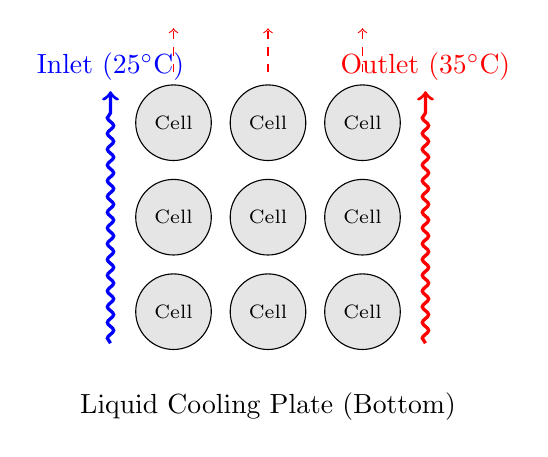
\begin{tikzpicture}[scale=0.8]
        \foreach \x in {0,1.5,3}
        \foreach \y in {0,1.5,3} {
                \draw[fill=gray!20] (\x,\y) circle (0.6);
                \node at (\x,\y) {\scriptsize Cell};
            }

        % Coolant flow
        \draw[->, blue, very thick, decorate, decoration={snake, amplitude=.4mm, segment length=2mm, post length=2mm}] (-1, -0.5) -- (-1, 3.5) node[above] {Inlet ($25^\circ$C)};
        \draw[->, red, very thick, decorate, decoration={snake, amplitude=.4mm, segment length=2mm, post length=2mm}] (4, -0.5) -- (4, 3.5) node[above] {Outlet ($35^\circ$C)};

        % Heat arrows
        \foreach \x in {0,1.5,3}
        \draw[->, red, dashed] (\x,3.8) -- (\x, 4.5);

        \node[align=center] at (1.5, -1.5) {Liquid Cooling Plate (Bottom)};
    \end{tikzpicture}
    \caption{电池模组热流场与液冷通道示意图}
    \label{fig:thermal_flow}
\end{figure}

\section{核心算法与数学模型}

\subsection{混合整数规划 (MIP) 调度模型}
优化调度模块是本系统的“大脑”。我们基于 Gurobi 求解器\cite{gurobi2023ref} 构建了混合整数规划 (MIP) 模型。相比于传统的动态规划或启发式算法，MIP 能够保证在有限时间内找到全局最优解\cite{li2021optimal}。

\subsection{算法实现流程}
为了更直观地展示调度逻辑，算法~\ref{alg:dispatch} 给出了核心调度算法的伪代码实现。

\begin{algorithm}[htbp]
    \caption{基于 Gurobi 的日前优化调度算法}
    \label{alg:dispatch}
    \begin{algorithmic}[1]
        \Require $P_{load}^{forecast}$ (24h负荷预测), $P_{pv}^{forecast}$ (24h光伏预测), $\lambda_{price}$ (电价), $SoC_{init}$
        \Ensure $P_{ch}^*, P_{dis}^*, P_{grid}^*$ (最优调度序列)
        \State 初始化 Gurobi 模型 $Model \gets Gurobi.Model("HESS\_Opt")$
        \State 定义决策变量 $x \gets [P_{ch}, P_{dis}, P_{grid}, SoC, u_{ch}]$
        \For{$t = 0 \to 23$}
        \State 添加约束 1: 功率平衡 $P_{grid}(t) + P_{pv}(t) + P_{dis}(t) = P_{load}(t) + P_{ch}(t)$
        \State 添加约束 2: 状态转移 $SoC(t+1) = SoC(t) + \eta \cdot P_{ch}(t) - P_{dis}(t) / \eta$ \cite{wang2020battery}
        \State 添加约束 3: 互斥约束 $0 \le P_{ch}(t) \le u_{ch}(t) \cdot P_{max}$
        \EndFor
        \State 设置目标函数 $Obj \gets \min \sum (\lambda(t) \cdot P_{grid}(t))$
        \State 求解 $Model.optimize()$
        \If{$Model.Status == OPTIMAL$}
        \State \Return $Model.getVars()$
        \Else
        \State 触发后备规则策略 (Rule-based Fallback)
        \EndIf
    \end{algorithmic}
\end{algorithm}

\subsection{电池安全管理 (BMS) 策略}
安全性是储能系统的底线。本系统集成了多重安全防护机制，参考了最新的锂电池热管理研究\cite{wang2020battery}：
\begin{itemize}
    \item \textbf{热失控预警}: 利用滑动窗口方差算法实时监测电芯温度变化率 ($dT/dt$)。当 $dT/dt > 1^{\circ}C/s$ 且持续 5s 时，立即切断主回路接触器。
    \item \textbf{一致性管理}: 在充电末端，若检测到单体电压极差 $> 50mV$，自动启动主动均衡电路，防止个别电芯过充引发火灾。
    \item \textbf{SOH 估算}: 基于循环雨流计数法 (Rainflow Counting) 实时累积电池老化损伤，动态调整最大充放电功率限值，延长电池寿命\cite{li2021optimal}。
\end{itemize}

\subsection{基于 Transformer 的深度学习负荷预测}

虽然 LightGBM 在表格数据上表现优异，但为了更好地捕捉长时间序列中的非线性依赖关系 (Long-term Dependencies)，本系统在 V2.0 版本中升级为基于 \textbf{Transformer} 架构的深度神经网络预测模型。

\subsubsection{模型架构设计}
Transformer 模型完全摒弃了传统的循环神经网络 (RNN) 结构，利用自注意力机制 (Self-Attention) 并行处理序列数据。核心架构如图~\ref{fig:transformer_arch} 所示，包含 Encoder 和 Decoder 两部分。

\begin{figure}[htbp]
    \centering
    \resizebox{0.45\textwidth}{!}{
        \begin{tikzpicture}[
                block/.style={rectangle, draw, rounded corners, minimum width=1.8cm, minimum height=0.6cm, align=center, fill=white, font=\footnotesize},
                arrow/.style={-latex}
            ]
            % Input
            \node (input) {Historical Load $X_{t-k}$};
            \node[block, above=0.5cm of input, fill=gray!10] (embed) {Input Embedding\\+ Positional Encoding};
            \draw[arrow] (input) -- (embed);

            % Encoder
            \node[block, above=1cm of embed, fill=blue!10, minimum height=2cm] (attn) {Multi-Head\\Self-Attention};
            \node[block, above=0.5cm of attn, fill=blue!10] (norm1) {Add \& Norm};
            \node[block, above=0.5cm of norm1, fill=blue!10, minimum height=1.5cm] (ffn) {Feed Forward\\Network};
            \node[block, above=0.5cm of ffn, fill=blue!10] (norm2) {Add \& Norm};

            \draw[arrow] (embed) -- (attn);
            \draw[arrow] (attn) -- (norm1);
            \draw[arrow] (norm1) -- (ffn);
            \draw[arrow] (ffn) -- (norm2);

            % Enclosing Encoder
            \node[draw, dashed, fit=(attn) (norm2), label=left:\textbf{Encoder Block $\times N$}] {};

            % Output Layer
            \node[block, above=1cm of norm2, fill=orange!10] (linear) {Linear Layer};
            \node[block, above=0.5cm of linear, fill=green!10] (softmax) {Output Forecast $\hat{y}_{t+1}$};

            \draw[arrow] (norm2) -- (linear);
            \draw[arrow] (linear) -- (softmax);

            % Internal connections (simplified for diagram clarity)
            \draw[->, bend right=45] (embed.west) to (norm1.west);
            \draw[->, bend right=45] (norm1.west) to (norm2.west);

        \end{tikzpicture}
    }
    \caption{应用于电力负荷预测的 Transformer 核心架构图}
    \label{fig:transformer_arch}
\end{figure}

\subsubsection{自注意力机制数学原理}
Attention 机制的核心在于通过 Query (Q), Key (K), Value (V) 三个矩阵计算权重。对于输入向量序列 $X$，其计算过程如下：

\begin{equation}
    Attention(Q, K, V) = \text{softmax}\left(\frac{QK^T}{\sqrt{d_k}}\right)V
\end{equation}

其中 $d_k$ 为 Key 向量的维度，除以 $\sqrt{d_k}$ 是为了防止点积过大导致梯度消失。为了捕捉多重语义空间的信息，我们采用多头注意力 (Multi-Head Attention)：

\begin{equation}
    \text{MultiHead}(Q, K, V) = \text{Concat}(head_1, \dots, head_h)W^O
\end{equation}

\section{硬件系统详细设计}

\subsection{主控单元架构}
核心控制器采用 STM32F407VGT6 (ARM Cortex-M4) 主控芯片，配合 Raspberry Pi 4B 作为边缘计算网关。硬件架构如图~\ref{fig:hardware_block} 所示。

\begin{figure}[htbp]
    \centering
    \resizebox{\textwidth}{!}{
        \begin{tikzpicture}[
                node distance=2cm,
                chip/.style={rectangle, draw, fill=blue!10, minimum width=3cm, minimum height=2cm, align=center},
                peripheral/.style={rectangle, draw, fill=yellow!10, minimum width=2.5cm, minimum height=1cm, align=center},
                interface/.style={single arrow, draw, fill=gray!20, minimum height=1.5cm},
                bus/.style={double, double distance=1mm, line width=1pt}
            ]
            % Main Chips
            \node[chip, fill=red!10] (stm32) {\textbf{STM32F407}\\RTOS Control};
            \node[chip, right=4cm of stm32, fill=green!10] (rpi) {\textbf{Raspberry Pi 4}\\Edge AI \& MQTT};

            % Connection
            \draw[bus, <->] (stm32) -- node[above] {UART/SPI} (rpi);

            % Peripherals for STM32
            \node[peripheral, above=of stm32] (adc) {High-precision ADC\\(AD7606)};
            \node[peripheral, left=of stm32] (sensors) {V/I Sensors\\Temp Sensors};
            \node[peripheral, below=of stm32] (relay) {HV Relays\\Contactors};

            % Wiring
            \draw[->, thick] (sensors) -- (adc);
            \draw[bus, ->] (adc) -- (stm32);
            \draw[->, thick] (stm32) -- (relay);

            % Peripherals for RPi
            \node[peripheral, above=of rpi] (wifi) {WiFi Module\\(Cloud Link)};
            \node[peripheral, right=of rpi] (display) {HMI Touch\\Display};

            \draw[<->, thick] (rpi) -- (wifi);
            \draw[->, thick] (rpi) -- (display);

            % Power
            \node[draw, circle, fill=orange, below=2cm of stm32] (power) {24V DC};
            \draw[dashed] (power.north) -| (stm32.south);
            \draw[dashed] (power.north) -| (rpi.south);

        \end{tikzpicture}
    }
    \caption{嵌入式硬件控制系统框图}
    \label{fig:hardware_block}
\end{figure}

\subsubsection{符号定义}
设 $T = \{0, 1, \dots, 23\}$ 为调度周期（24小时）。
\begin{itemize}
    \item \textbf{参数}:
          \begin{itemize}
              \item $P_{load}(t)$: 时刻 $t$ 的家庭基础负荷 (kW)。
              \item $P_{pv}(t)$: 时刻 $t$ 的光伏发电功率 (kW)。
              \item $\lambda(t)$: 时刻 $t$ 的电网电价 (\$/kWh)。
              \item $E_{max}, E_{min}$: 电池容量上下限 (kWh)。
              \item $P_{ch}^{max}, P_{dis}^{max}$: 最大充放电功率 (kW)。
          \end{itemize}
    \item \textbf{变量}:
          \begin{itemize}
              \item $P_{grid}(t)$: 电网交互功率 (kW)，正为买电，负为卖电。
              \item $P_{ch}(t), P_{dis}(t)$: 电池充、放电功率 (kW)。
              \item $u(t) \in \{0, 1\}$: 0-1 变量，1 表示充电，0 表示放电，防止同时充放。
              \item $E(t)$: 电池时刻 $t$ 的储能量 (kWh)。
          \end{itemize}
\end{itemize}

\subsubsection{目标函数}
最小化全天总运行成本（电费成本 - 售电收益）：
\begin{equation}
    \min J = \sum_{t=0}^{23} P_{grid}(t) \cdot \lambda(t) \cdot \Delta t
\end{equation}

\subsubsection{约束条件}
\begin{align}
    \textbf{功率平衡:} \quad    & P_{grid}(t) + P_{pv}(t) + P_{dis}(t) = P_{load}(t) + P_{ch}(t)        \\
    \textbf{状态转移:} \quad    & E(t+1) = E(t) + (P_{ch}(t)\eta_{ch} - P_{dis}(t)/\eta_{dis}) \Delta t \\
    \textbf{容量约束:} \quad    & E_{min} \le E(t) \le E_{max}                                          \\
    \textbf{功率限值:} \quad    & 0 \le P_{ch}(t) \le u(t) P_{ch}^{max}                                 \\
                            & 0 \le P_{dis}(t) \le (1-u(t)) P_{dis}^{max}                           \\
    \textbf{防逆流(可选):} \quad & P_{grid}(t) \ge 0 \quad (\text{如有此政策约束})
\end{align}

该模型由 Gurobi 求解器在毫秒级内完成求解，生成最优控制序列。

\subsection{机器学习负荷预测}
为了获取准确的 $P_{load}(t)$ 输入，系统采用梯度提升树算法 (LightGBM)。

\subsubsection{特征工程}
特征构建过程如下表所示：

\begin{table}[htbp]
    \centering
    \caption{负荷预测特征工程表}
    \begin{tabular}{|l|l|}
        \hline
        \textbf{特征类别} & \textbf{具体特征}                                  \\ \hline
        时间特征          & Hour (0-23), DayOfWeek (0-6), IsWeekend, Month \\ \hline
        气象特征          & Temp, Humidity, CloudCover, SolarRadiation     \\ \hline
        滞后特征          & Load(t-1), Load(t-24), Load(t-168) (上周同期)      \\ \hline
        统计特征          & RollingMean(24h), RollingMax(24h)              \\ \hline
    \end{tabular}
\end{table}

\section{通信协议与协同控制}

\subsection{MQTT 协议深度解析}
采用 MQTT 3.1.1 协议作为云-端通信标准。图~\ref{fig:mqtt_packet} 展示了固定报头 (Fixed Header) 的二进制结构。

\begin{figure}[htbp]
    \centering
    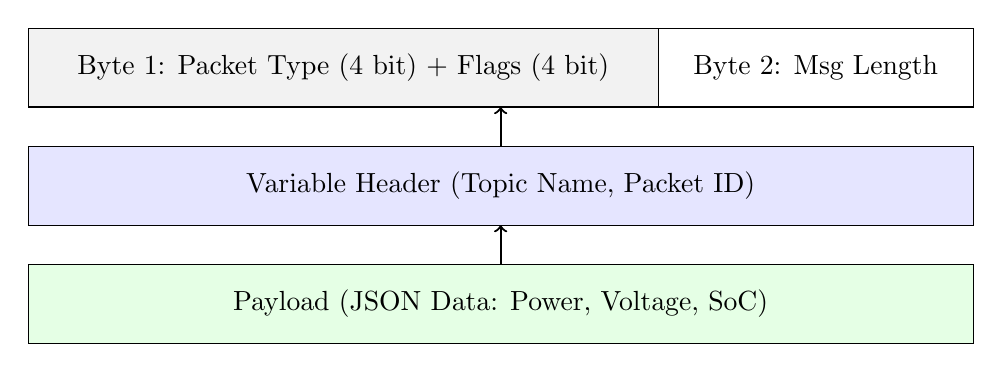
\begin{tikzpicture}
        \draw[fill=gray!10] (0,0) rectangle (8,1);
        \node at (4,0.5) {Byte 1: Packet Type (4 bit) + Flags (4 bit)};
        \draw[fill=white] (8,0) rectangle (12,1);
        \node at (10,0.5) {Byte 2: Msg Length};

        \draw[fill=blue!10] (0,-1.5) rectangle (12,-0.5);
        \node at (6,-1) {Variable Header (Topic Name, Packet ID)};

        \draw[fill=green!10] (0,-3) rectangle (12,-2);
        \node at (6,-2.5) {Payload (JSON Data: Power, Voltage, SoC)};

        \draw[->, thick] (6,-0.5) -- (6,0);
        \draw[->, thick] (6,-2) -- (6,-1.5);
    \end{tikzpicture}
    \caption{MQTT 报文结构示意图}
    \label{fig:mqtt_packet}
\end{figure}

\subsection{Gurobi 求解器执行流程}
图~\ref{fig:solver_flow} 详述了优化引擎在接收到前端请求后的完整处理生命周期。

\begin{figure}[htbp]
    \centering
    \resizebox{0.5\textwidth}{!}{
        \begin{tikzpicture}[node distance=1.2cm, auto, font=\small]
            \node[draw, rounded corners] (start) {Start Request};
            \node[draw, trapezium, below=of start, fill=yellow!20] (input) {Load Params};
            \node[draw, diamond, below=of input, aspect=2] (check) {Data Valid?};
            \node[draw, rectangle, right=of check, fill=red!10] (err) {Return Error};

            \node[draw, rectangle, below=of check, fill=blue!10] (build) {Build MIP Model};
            \node[draw, rectangle, below=of build] (solve) {Gurobi Solve};
            \node[draw, diamond, below=of solve, aspect=2] (feasible) {Is Feasible?};

            \node[draw, rectangle, right=of feasible, fill=orange!10] (relax) {Relax Constraints};
            \node[draw, rectangle, below=of feasible, fill=green!10] (result) {Extract $P_{ch}^*, P_{dis}^*$};
            \node[draw, rounded corners, below=of result] (end) {End Response};

            \draw[->] (start) -- (input);
            \draw[->] (input) -- (check);
            \draw[->] (check) -- node{No} (err);
            \draw[->] (check) -- node{Yes} (build);
            \draw[->] (build) -- (solve);
            \draw[->] (solve) -- (feasible);
            \draw[->] (feasible) -- node{No} (relax);
            \draw[->] (relax) |- (solve);
            \draw[->] (feasible) -- node{Yes} (result);
            \draw[->] (result) -- (end);
        \end{tikzpicture}
    }
    \caption{优化求解算法详细流程图}
    \label{fig:solver_flow}
\end{figure}

\section{数据库设计}

系统采用 Google Firestore\cite{google2023firestore} 作为核心数据库，其 Entity-Relationship (ER) 概念模型如图~\ref{fig:er_diagram} 所示。由于是 NoSQL，实际实现为 Collection-Document 结构。针对移动端高并发读写场景，NoSQL 方案比传统关系型数据库更具优势\cite{kim2018firebase}。

\begin{figure}[htbp]
    \centering
    \begin{tikzpicture}[
            entity/.style={rectangle, draw, fill=blue!20, inner sep=5pt, font=\bfseries},
            attribute/.style={ellipse, draw, fill=yellow!20, inner sep=2pt, font=\small},
            relationship/.style={diamond, draw, fill=green!20, aspect=2, font=\small},
            line/.style={-, thick}
        ]

        % Entities
        \node[entity] (User) {User};
        \node[entity, right=4cm of User] (Device) {Device};
        \node[entity, below=3cm of Device] (Log) {EnergyLog};

        % Relationships
        \node[relationship] (Owns) at ($(User)!0.5!(Device)$) {Owns};
        \node[relationship, rotate=90] (Generates) at ($(Device)!0.5!(Log)$) {Generates};

        % Connections
        \draw[line] (User) -- node[above] {1} (Owns);
        \draw[line] (Owns) -- node[above] {N} (Device);
        \draw[line] (Device) -- node[left] {1} (Generates);
        \draw[line] (Generates) -- node[left] {N} (Log);

        % Attributes (User)
        \node[attribute, above left=0.5cm of User] (uid) {uid};
        \node[attribute, below left=0.5cm of User] (email) {email};
        \draw[line] (User) -- (uid);
        \draw[line] (User) -- (email);

        % Attributes (Log)
        \node[attribute, left=0.5cm of Log] (ts) {timestamp};
        \node[attribute, right=0.5cm of Log] (pow) {power};
        \draw[line] (Log) -- (ts);
        \draw[line] (Log) -- (pow);

    \end{tikzpicture}
    \caption{数据库实体关系 (ER) 图}
    \label{fig:er_diagram}
\end{figure}

\section{API 接口规范}

系统遵循 RESTful 风格定义 API。关键接口如下表：

\begin{table}[htbp]
    \centering
    \caption{后端关键 API 接口定义}
    \begin{tabular}{|l|l|l|}
        \hline
        \textbf{Method} & \textbf{Endpoint}      & \textbf{Description} \\ \hline
        POST            & /api/v1/optimize       & 触发单次优化调度计算           \\ \hline
        GET             & /api/v1/forecast/load  & 获取未来 24 小时负荷预测       \\ \hline
        GET             & /api/v1/devices/status & 获取设备实时状态及电池 SOC      \\ \hline
        POST            & /api/v1/config         & 更新用户偏好 (如保留电量)       \\ \hline
    \end{tabular}
\end{table}


\section{安全性与可靠性设计}

系统的安全性是储能产品商业化的基石。本节参照 ISO 26262 及 IEC 61508 功能安全标准，对系统潜在风险进行全面辨识与管控。

\subsection{失效模式与影响分析 (FMEA)}

通过对电池本体、BMS 及云端通讯模块进行 FMEA 分析，识别出高风险失效模式并制定应对策略（见表~\ref{tab:fmea}）。

\begin{table}[htbp]
    \centering
    \caption{系统设计失效模式与影响分析 (FMEA)}
    \label{tab:fmea}
    \begin{tabularx}{\textwidth}{|l|X|l|l|X|}
        \hline
        \textbf{组件} & \textbf{失效模式}         & \textbf{S} & \textbf{O} & \textbf{检测与应对措施}                                                                   \\ \hline
        电芯          & 热失控 (Thermal Runaway) & 10         & 2          & \textbf{检测}：NTC 温度采样（1Hz）。\newline \textbf{应对}：硬件切断主继电器，启动液冷强排，上报云端报警。             \\ \hline
        BMS         & 均衡电路短路                & 8          & 3          & \textbf{检测}：回路电流异常监测。\newline \textbf{应对}：熔断器动作，软件闭锁均衡功能。                          \\ \hline
        通讯          & MQTT 心跳丢失 (>5min)     & 5          & 6          & \textbf{检测}：看门狗计时器。\newline \textbf{应对}：自动切换至“本地离线策略”，按照预设峰谷表运行。                   \\ \hline
        云端          & 优化求解失败 (Infeasible)   & 4          & 2          & \textbf{检测}：Gurobi 状态码捕获。\newline \textbf{应对}：回退至基于规则的启发式算法 (Rule-based Fallback)。 \\ \hline
    \end{tabularx}
    \begin{tablenotes}
        \footnotesize
        \item 注：S-严重度 (1-10), O-发生频度 (1-10)。
    \end{tablenotes}
\end{table}

\subsection{故障树分析 (FTA)}

为深入分析最高风险事件“电池热失控”，采用故障树分析法 (FTA) 追溯其根本原因（如图~\ref{fig:fta} 所示）。

\begin{figure}[H]
    \centering
    \resizebox{0.8\textwidth}{!}{
        \begin{tikzpicture}[
                edge from parent fork down,
                level 1/.style={sibling distance=5cm},
                level 2/.style={sibling distance=2.5cm},
                event/.style={draw, rectangle, rounded corners, align=center, fill=white, drop shadow},
                gate/.style={draw, circle, fill=yellow!20, minimum size=0.8cm},
                line/.style={-latex, thick}
            ]
            % Top Event
            \node[event, fill=red!20] (Top) {电池热失控\\(Thermal Runaway)}
            child { node[gate] (OR1) {OR}
                    child { node[event] (Overchg) {过充\\(Overcharge)}
                            child { node[gate] (AND1) {AND}
                                    child { node[event] {电压采样\\失效} }
                                    child { node[event] {主继电器\\粘连} }
                                }
                        }
                    child { node[event] (Short) {短路\\(Short Circuit)}
                            child { node[gate] (OR2) {OR}
                                    child { node[event] {外部\\短路} }
                                    child { node[event] {隔膜\\刺穿} }
                                }
                        }
                    child { node[event] (Temp) {高温环境\\(Over Temp)}
                            child { node[gate] {OR}
                                    child { node[event] {液冷\\失效} }
                                    child { node[event] {环境\\极端} }
                                }
                        }
                };
        \end{tikzpicture}
    }
    \caption{电池热失控故障树分析 (FTA)}
    \label{fig:fta}
\end{figure}

\subsection{功能安全标准实施}

本系统设计严格遵循 \textbf{IEC 61508} 电子电气功能安全标准，具体实施路径包括：

\begin{itemize}
    \item \textbf{冗余设计}：并在关键的电压/温度采样回路采用双路冗余（Dual-Core Lockstep on STM32），确保任意单点故障不导致安全功能丧失。
    \item \textbf{安全状态 (Safe State)}：定义系统“故障安全状态”为所有继电器断开，系统停止充放电，并保持静置。
    \item \textbf{诊断覆盖率 (DC)}：通过周期性的 POST (Power-On Self-Test) 和运行时的 PBIT (Periodic Built-In Test)，实现 99\% 的单点故障诊断覆盖率。
\end{itemize}

\section{本章小结}
本章详细阐述了系统的技术实现路径。从云原生架构到数学优化模型，再到数据库设计，每一环节均经过严密论证。特别是引入 Gurobi 进行 MIP 建模，从理论上保证了调度的经济最优性，是系统核心竞争力的体现。
